\section{Technical Conditions for Production} \label{sec:TechCon}

\subsection{Workshop Site Sizes}
Due to that, all the parts of the seat are bought from our suppliers, the workshop site size is mainly composed of the inventory and the assembly line. For a batch of 100 pieces, the parts need to prepare should be enough for 105 pieces.

Consider the stacking height limit for each layer is 2 meters and the width and the length are also 2 meters, and the storage structure is three layers, as shown in Figure \ref{fig:stocking structure}.

\begin{figure}[!htp]
    \centering
    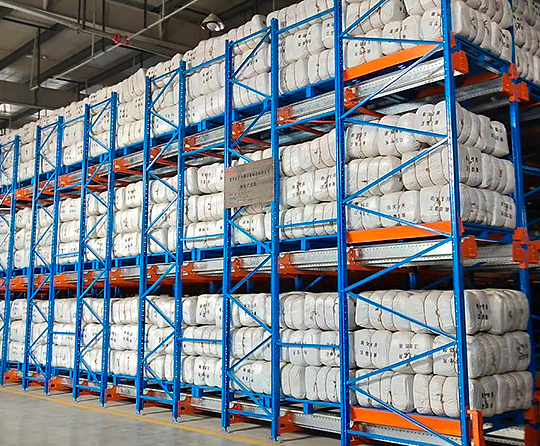
\includegraphics[width=0.6\textwidth]{images/stocking structure.jpg}
    \caption{Stocking Structure}
    \label{fig:stocking structure}
\end{figure}

For each stocking unit with a volume of 2m x 2m x 2m, the number of parts that can be stored is listed in Table \ref{tab:stocking unit}.

\begin{table}[!htp]
    \centering
    \caption{The upper limit of the number of each part that can be stored in one stocking unit}
    \label{tab:stocking unit}
    \begin{tabular}{cccc} \toprule
        Name                   & Volume ($\mathrm{m^3}$) & Storage limit & Need \\
        \midrule
        Leg                    & 0.00076368                    & 10475    & 840  \\
        Seat frame             & 0.011746428                   & 681      & 105  \\
        Backrest frame         & 0.017965125                   & 445      & 105  \\
        Headrest frame         & 0.003553541                   & 2251     & 105  \\
        Seat Assembly          & 0.021172087                   & 377      & 105  \\
        Headrest Assembly      & 0.003553541                   & 2251     & 105  \\
        Backrest Assembly      & 0.028972329                   & 276      & 105  \\
        Armrests               & 0.0008001                     & 9998     & 210  \\
        Foldable desk assembly & 0.000193548                   & 41333    & 210  \\
        \bottomrule
    \end{tabular}
\end{table}

It can be found that the number of parts that can be stored in one stocking unit is far more than the number of parts needed for a batch of 100 pieces. Therefore, the storage space is sufficient. Suppose we store each part in independent stocking units, also consider one workbench for all the screws and fasteners and three -more stocking units for the assembled seats, the total number of stocking units needed is 12. The inventory size would be the area of the workbench, four three-layer stocking structures and the aisles. Therefore, the inventory size is $S_\mathrm{inventory}=12\times16=192\mathrm{m^2}$, which includes a very large margin for passage and logistics.

To assemble such a product, an assembly line would need to be established with different stations for each component. Below is a suggested assembly line process:

\begin{enumerate}
    \item Frame assembly station - Assemble the aluminum legs and plastic frames (SF-001, SF-002, SF-003, SF-004) to form the seat frame structure.
    
    \item  Recline mechanism installation station - Install the recline mechanism (SF-005) onto the seat frame.
    
    \item  Cushion installation station - Install the polyurethane foam cushions (SC-001, HR-001, BR-001) onto the plastic frames.
    
    \item  Armrest and desk assembly station - Assemble the molded plastic armrests (AR-001) and foldable desk assembly (FD-001) onto the seat frame.
    
    \item Final assembly station - Attach the buttons (CF-001) to connect the cushions and covers, and fasten all components with screws (CF-002), bolts (CF-003), nuts (CF-004), and washers (CF-005) using appropriate tools. Attach the hinges (CF-006) to the foldable desk assembly.
\end{enumerate}

Assuming that each station will require a workspace of at least three times the size of the largest component, the assembly line will require a space of at least $1.9812 \times 1.2954 = 2.566\mathrm{m^2}$ for each station. Therefore, the total space required for the assembly line will be at least $2.566\times5=12.83\mathrm{m^2}$ for the five stations listed above. Additionally, there should be space for the workers to move around and transport the components from one station to another. Thus, the final assembly line space would be at least $25\mathrm{m^2}$.

Moreover, consider the stage of quality check, which will be introduced in Section \ref{sec:QC}, the space for the quality check is $S_\mathrm{QC}=1.5S_\mathrm{assembly line}=37.5\mathrm{m^2}$.

In all, the workshop site size is $S_\mathrm{workshop}=S_\mathrm{inventory}+S_\mathrm{assembly line}=192+25+37.5=254.5\mathrm{m^2}$. (Exclude the other Facilities that will be introduced in Section \ref{sec:Facilities} that are not directly related to the production process.)


\subsection{Consumables}
\subsubsection{Electricity}
According to industry sources, the electricity consumption of a typical sewing machine ranges from 200 to 400 watts per hour, while a cutting machine can consume up to 2,000 watts per hour. The power consumption of an assembly robot would depend on its size and capabilities.

Assuming an average power consumption of 500 watts per hour per machine, and an average of 20 machines in operation at any given time, the assembly line would require a total power supply of 10,000 watts per hour, or 10 kilowatts per hour (kWh). This translates to a daily consumption of 240 kWh (10 kW x 24 hours), assuming the line operates 24 hours a day.

Assuming an average lighting power density of 11 watts per square meter, the electricity consumption for lighting the inventory area would be 2,387 watts per hour, or 2.387 kWh. This translates to a daily consumption of 57.3 kWh (2.387 kW x 24 hours), assuming the lights are on 24 hours a day.

Therefore, the total daily electricity consumption of the workshop would be 297.3 kWh (240 kWh + 57.3 kWh).

\subsubsection{Water}
Assuming that each stage of the assembly line requires water for cooling and cleaning and that each stage uses about 10 liters of water per day, the total water consumption per day would be 5 stages x 10 liters/stage = 50 liters/day.

\subsubsection{Lubricants}
Assuming that each stage of the assembly line requires lubricants for machinery and equipment and that each stage uses about 0.5 liters of lubricants per day, the total lubricant consumption per day would be 5 stages x 0.5 liters/stage = 2.5 liters/day.

\subsubsection{Office supplies}
Assuming that each office employee needs about 5 sheets of paper, 1 ink cartridge, and 2 pens per day and that there are 2 office employees working each day, the total office supply consumption per day would be 2 employees x (5 sheets + 1 ink cartridge + 2 pens) = 14 units/day.

\subsection{Other Facilities Needed} \label{sec:Facilities}
Forklifts, as shown in Figure \ref{fig:forklift}, are needed for logistics, such as loading products or transporting parts and products between the inventory and the assembly line. Besides, for the sake of humanitarianism, a restroom and a break room are designed for the workers. The restroom should be equipped with a toilet, a sink, and a hand dryer. The break room should be equipped with a refrigerator, a microwave, a water dispenser, and a sofa. 

\begin{figure}
    \centering
    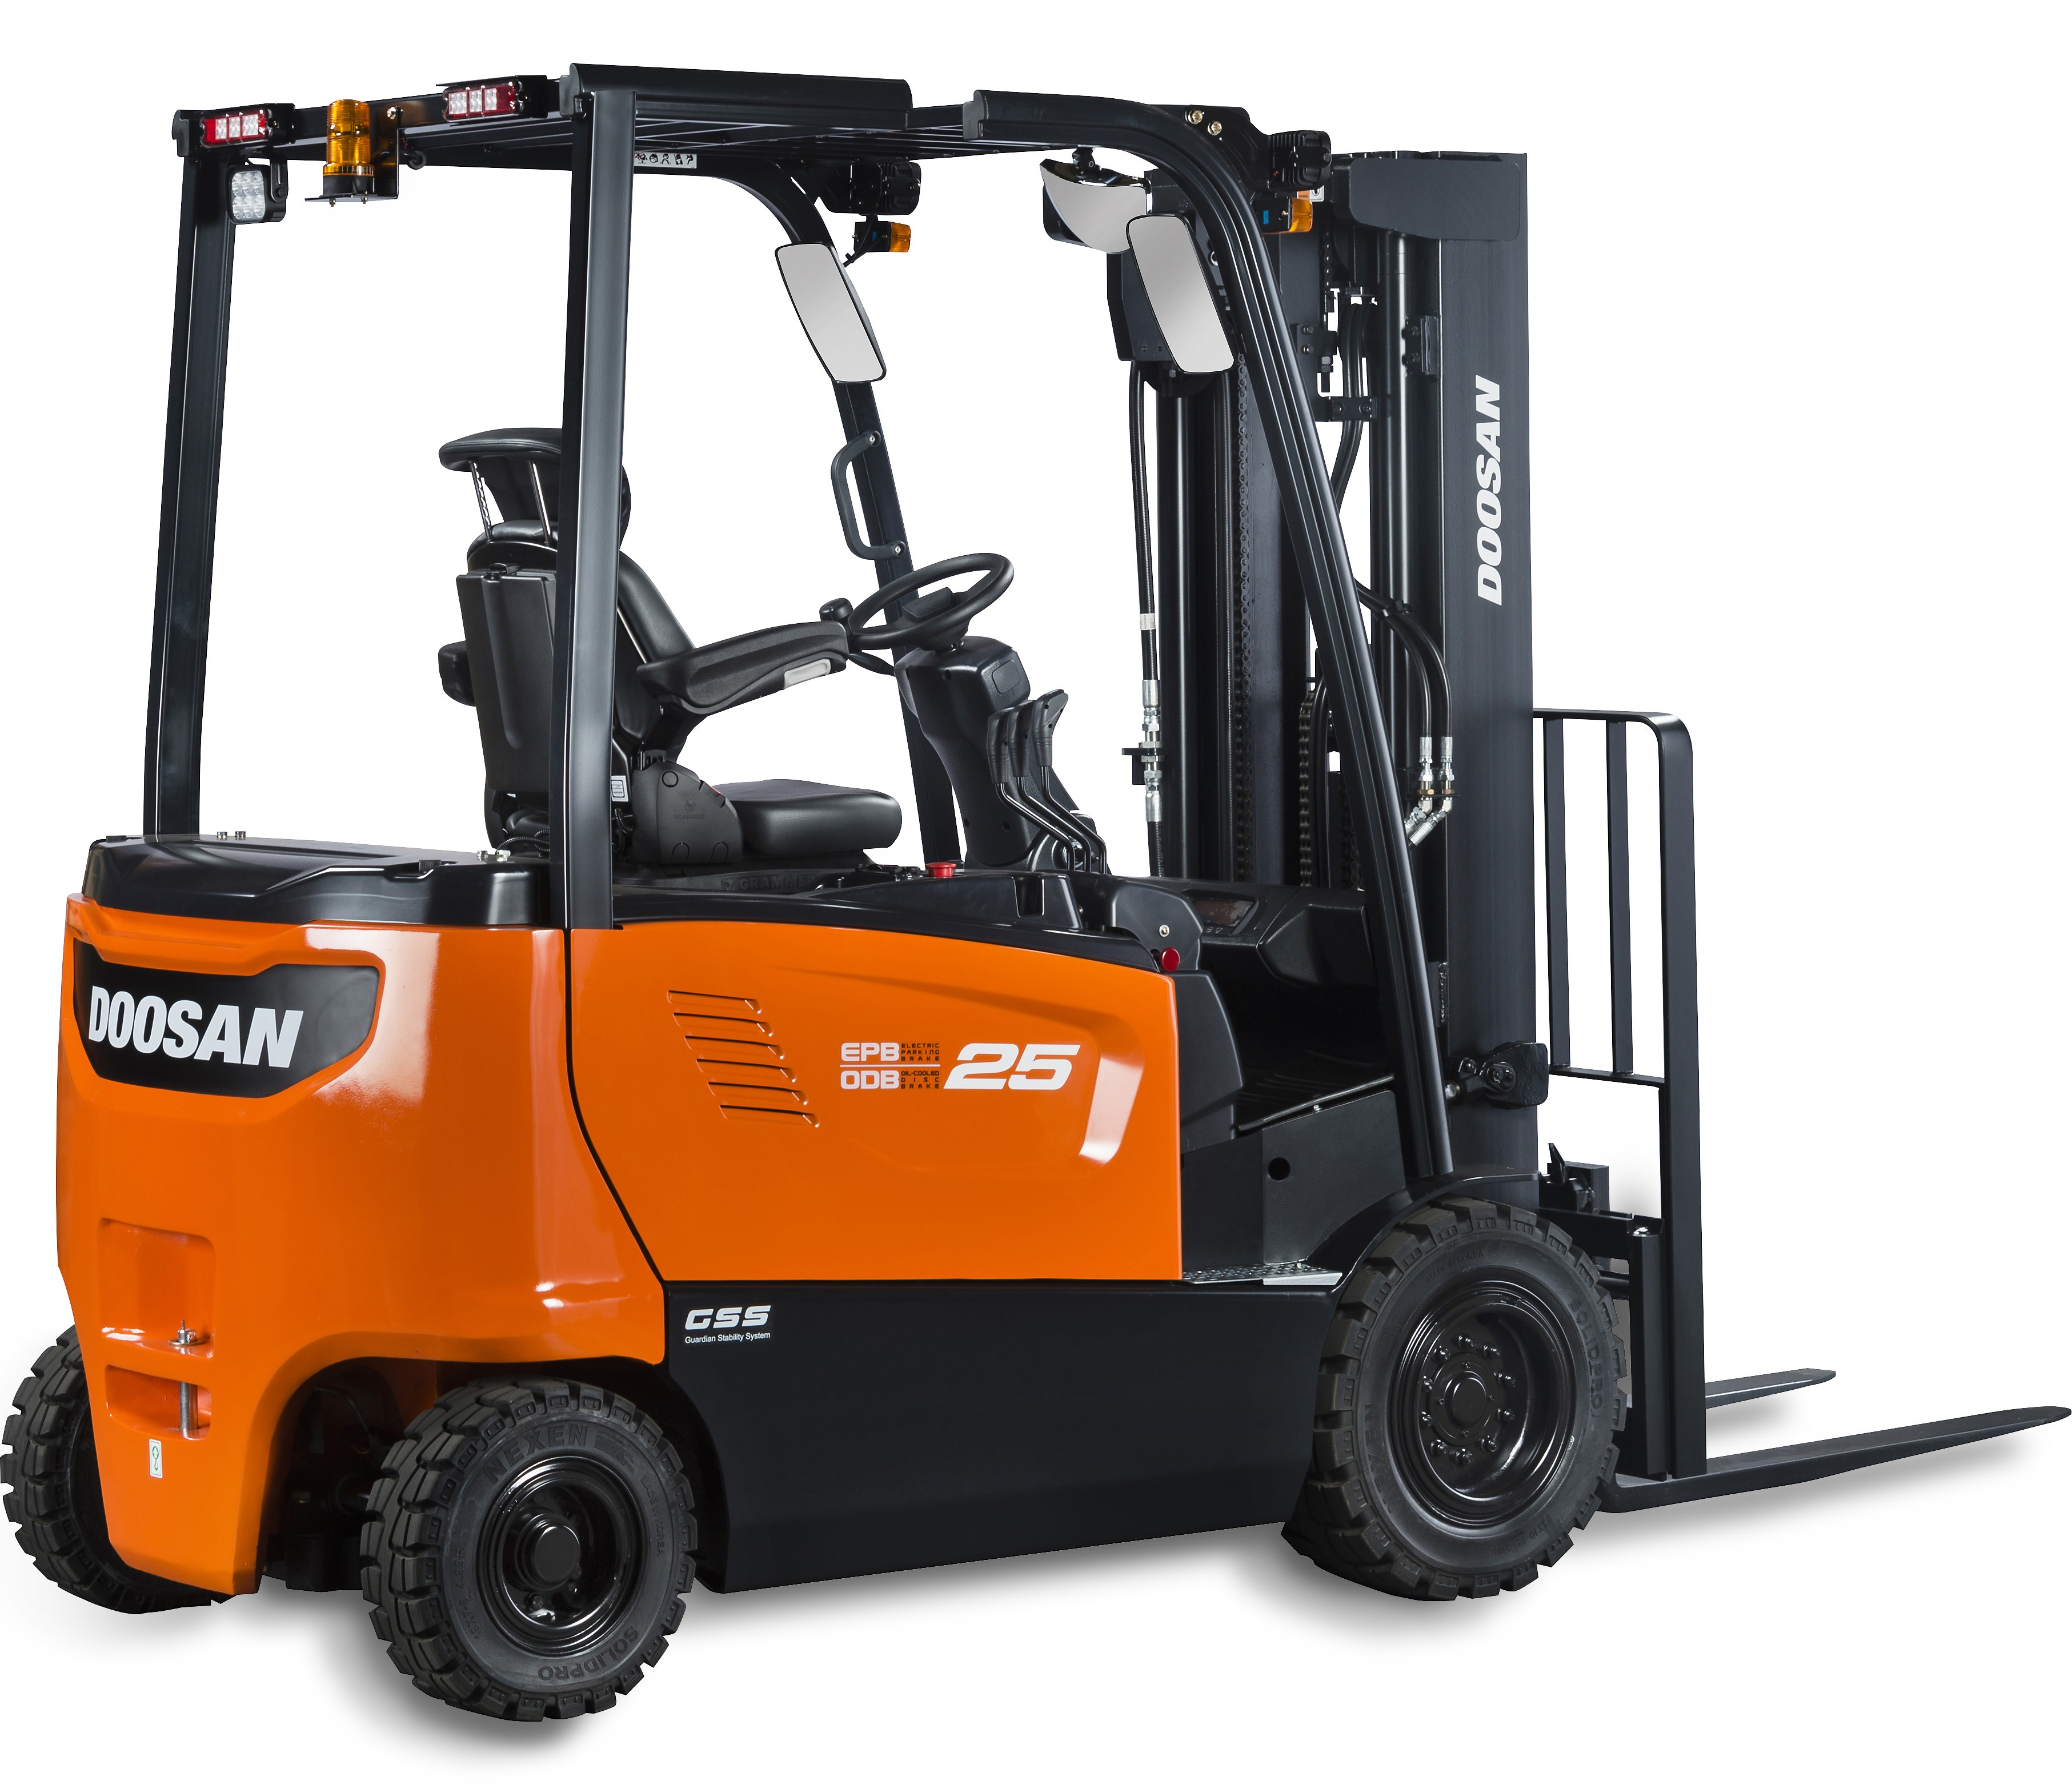
\includegraphics[width=0.8\textwidth]{images/forklift.jpg}
    \caption{Forklift}
    \label{fig:forklift}
\end{figure}


\subsection{Safety Measures}
\begin{enumerate}
    \item Training - All workers involved in the assembly line process and the inventory should undergo proper training on how to safely operate machinery, handle tools, follow safety procedures, handle materials and use equipment safely.
    \item Personal protective equipment (PPE) - Workers should wear appropriate PPE such as gloves, eye protection, ear protection, and steel-toed boots to protect them from potential hazards.
    \item Machine guarding - Machinery used in the assembly line should be properly guarded to prevent workers from accidentally coming into contact with moving parts.
    \item Material handling equipment - Equipment used for transporting and storing inventory such as forklifts, pallet jacks, and ladders should be properly maintained and operated according to safety standards.
    \item Ergonomics - Workstations should be designed to promote good posture and reduce the risk of repetitive strain injuries.
    \item First aid and emergency response - A first aid kit should be readily available, and workers should be trained on emergency response procedures in case of an accident or injury. Also, fire prevention measures should be in place such as having fire extinguishers, smoke detectors, and proper storage of flammable materials.
    \item Housekeeping - Good housekeeping practices should be followed to keep the inventory storage area clean and free from clutter, which can lead to tripping hazards.
    \item Regular maintenance and inspection - Regular maintenance and inspection of machinery and equipment should be conducted to ensure they are functioning correctly and do not pose a hazard to workers.
\end{enumerate}

\subsection{Factory Site Structure}
Based on the depiction in this section, the factory site structure is shown in Figure \ref{fig:factory_site_structure}.

\begin{figure}
    \centering
    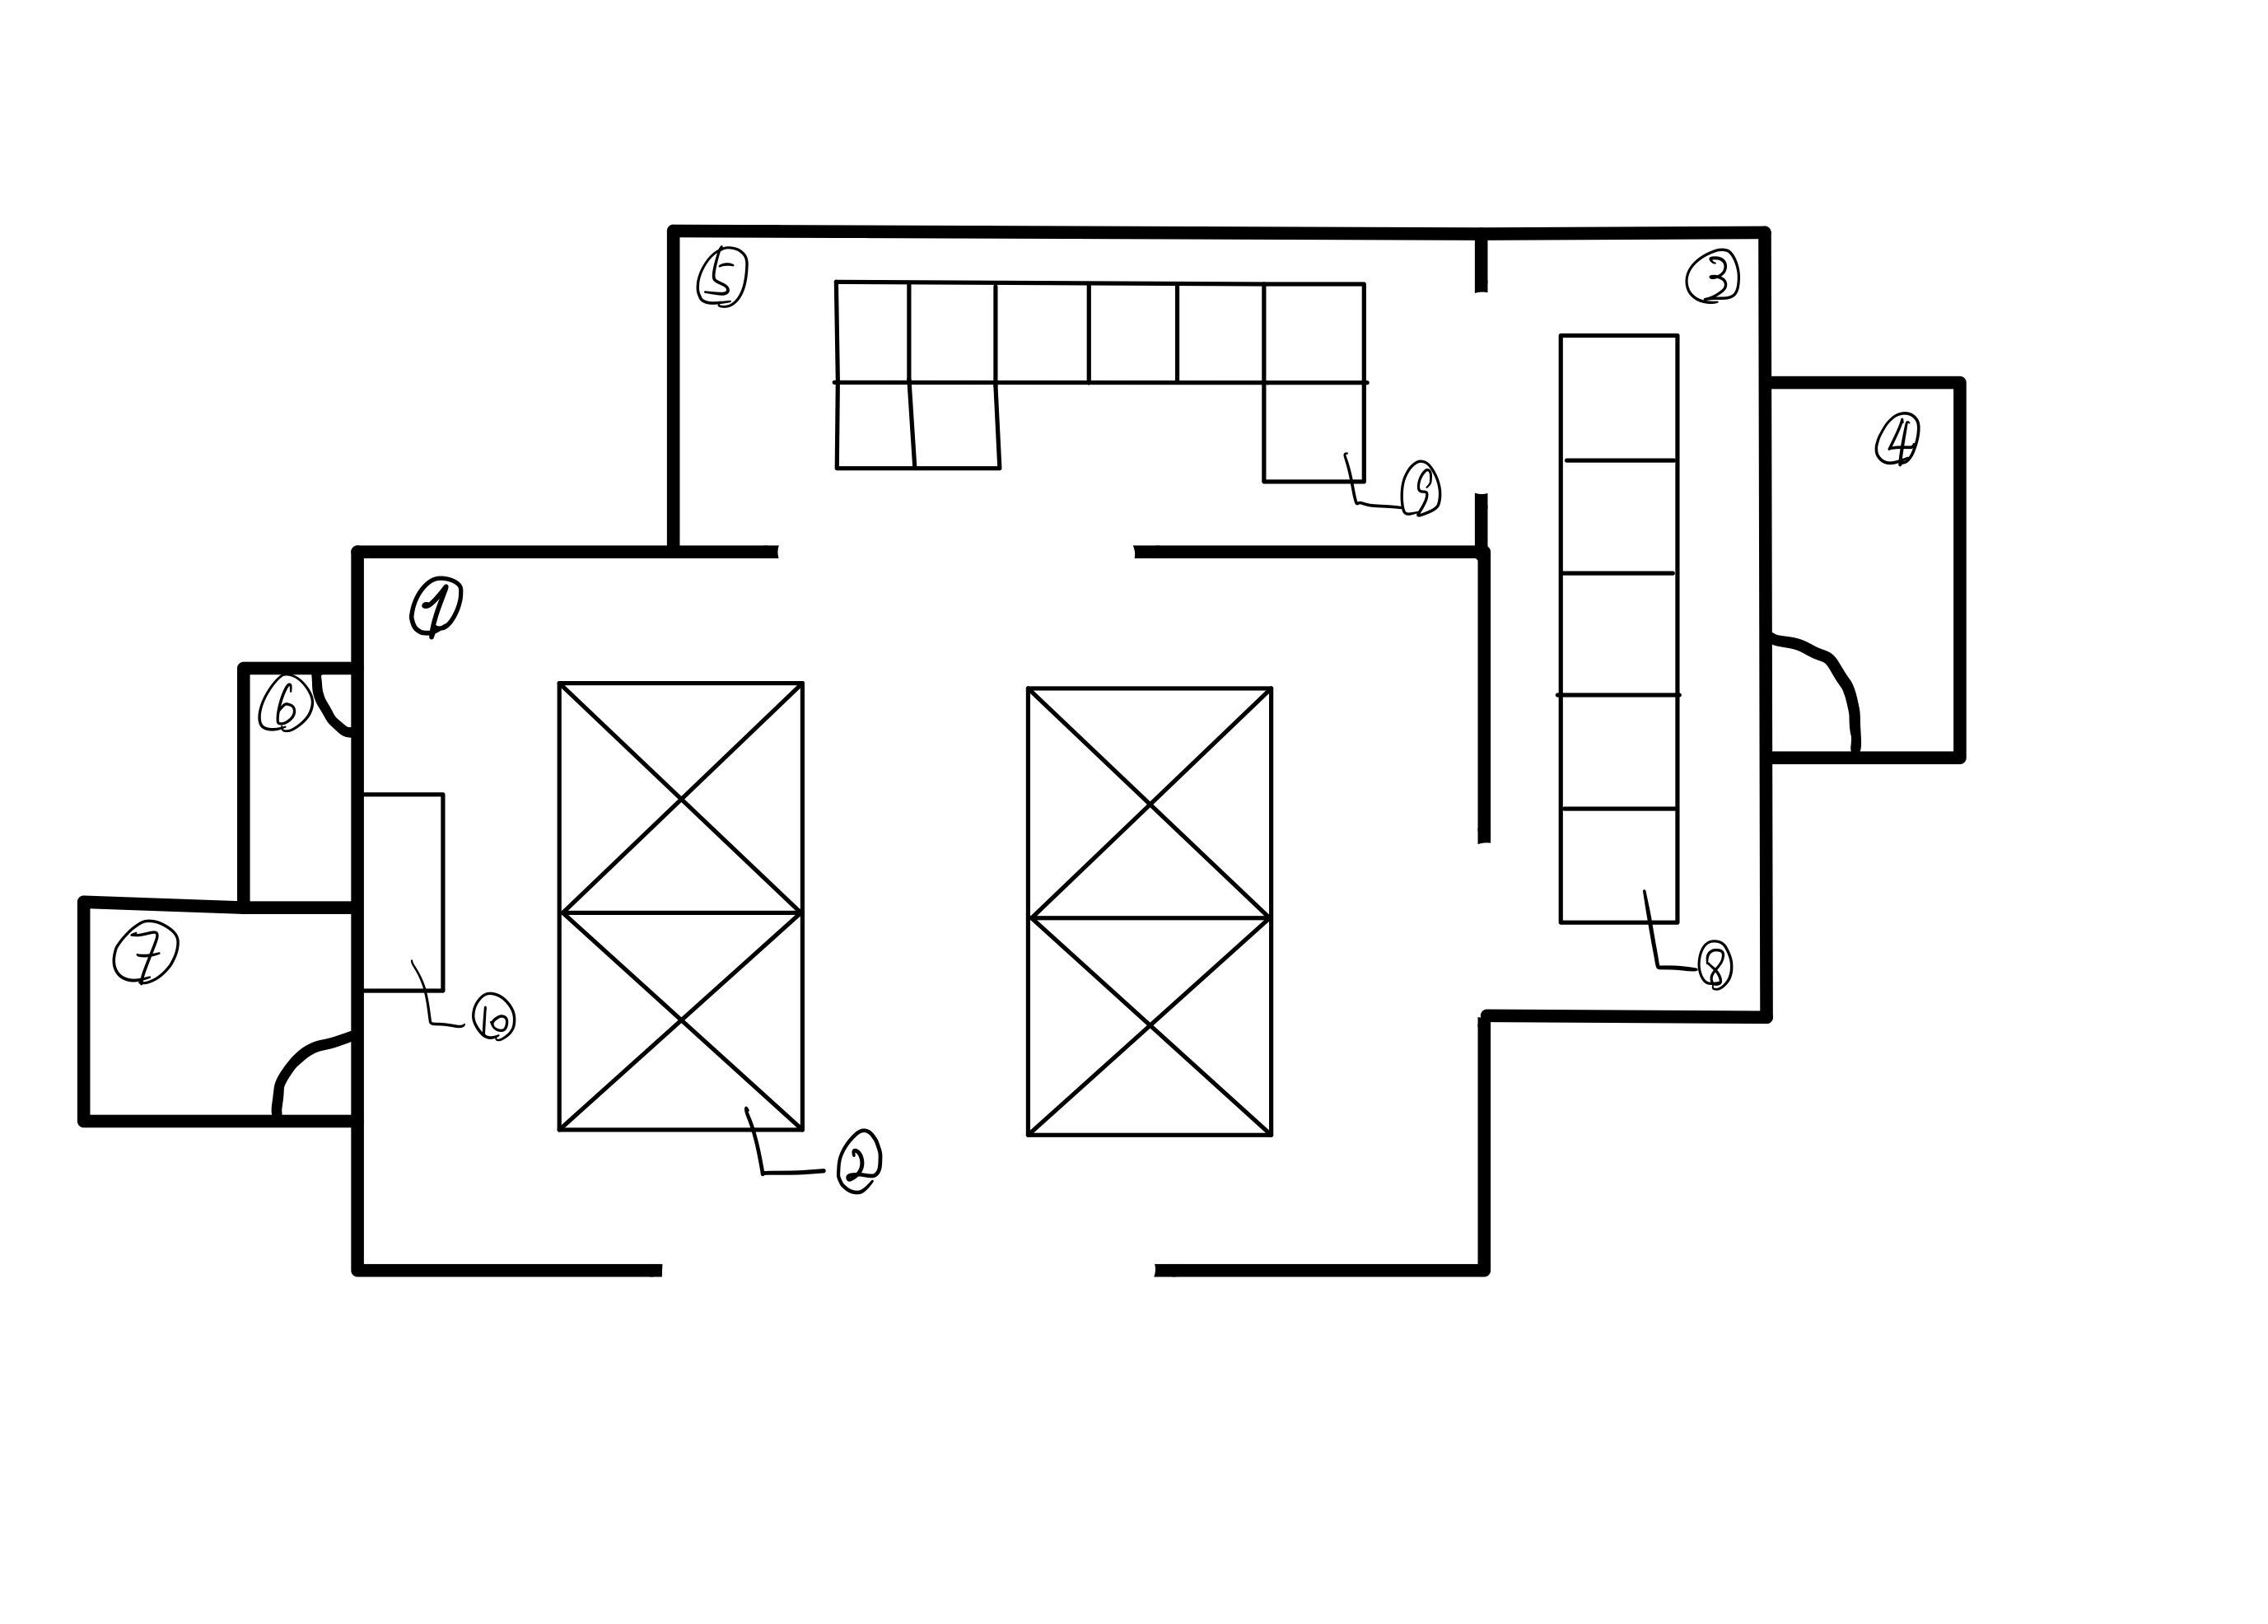
\includegraphics[width=\textwidth]{images/factory.jpg}
    \caption{Factory Site Structure}
    \label{fig:factory_site_structure}
\end{figure}

\textcircled{1}: Inventory.
\textcircled{2}: Stocking structure.
\textcircled{3}: Assembly room.
\textcircled{4}: Employee office (the furniture such as the desks is not shown in the figure).
\textcircled{5}: Quality check room.
\textcircled{6}: Restroom (the furniture such as the toilet is not shown in the figure).
\textcircled{7}: Break room (the furniture such as the sofa is not shown in the figure).
\textcircled{8}: Assembly line with 5 stations.
\textcircled{9}: Quality check stations with 9 stages.
\textcircled{10}: Workbench storing the screws and fasteners.